\documentclass{article}
\usepackage{nips15submit_e,times}
\usepackage{hyperref}
\usepackage{url}
\usepackage{graphicx}
\usepackage{booktabs}
\usepackage{float}

\hypersetup{colorlinks=true,urlcolor=blue,citecolor=blue,linkcolor=blue}

\title{Automated Digitization of Hand-Drawn Electrical\\ Schematics Using Computer Vision}

\author{
  Depanshu Suyal \quad Evan Wushke \quad Amtoj Punia \\
  \\
  Department of Mathematics and Computing \\
  Mount Royal University \\
}

\nipsfinalcopy

\begin{document}

\maketitle

\begin{abstract}
We present an end-to-end pipeline for automatically converting 
photographs of hand-drawn electrical schematics into clean, 
machine-readable diagrams. Our system composes three trained models 
in sequence: a YOLOv8m object detector for component localization, 
a ResNet-50 U-Net for wire segmentation, and a fine-tuned TrOCR 
transformer for handwritten label recognition, followed by a 
rule-based reconstruction stage that assembles a clean schematic 
from their outputs. Evaluated on the CGHD1152 dataset of 3{,}269 
annotated schematic photographs, the detector achieves mAP@0.50 
of 0.932 (precision 0.956, recall 0.910) across 62 classes, and 
the wire segmenter reaches 99.14\% pixel accuracy with a Dice score 
of 0.91. OCR with a character match accuracy of 0.95.
Code and trained models are available at 
\url{https://github.com/ewush956/Computer-Vision-Schematic-Parser}.
\end{abstract}

\section{Introduction}

Hand-drawn schematics remain common in circuit prototyping, education,
and field engineering, yet digitization is still largely manual: engineers
retrace drawings into tools such as KiCad by hand. Automated recognition of \emph{printed} or CAD-generated schematics 
is well studied~[5], but hand-drawn inputs introduce additional 
challenges: stroke imprecision, per-drafter symbol variation, 
handwritten labels, and perspective distortion from handheld cameras. 
Prior work on hand-drawn diagram recognition~[6] has addressed some 
of these, but at smaller scale and without the full digitization 
pipeline that practical use requires.

Bayer~[1] recently released CGHD1152, a large-scale annotated
dataset of hand-drawn electrical schematics. We use this dataset to
train three distinct models, each targeting one subproblem with a
suitable architecture, and compose them with a rule-based
reconstruction stage.

After most of our design was implemented, we became aware of the
closely related modular graph-extraction pipeline of Bayer et al.~[8],
which addresses the same problem with a similar decomposition. Our
project is an independent implementation with different model choices
(YOLOv8m vs.\ their faster R-CNN; TrOCR vs.\ their Tesseract stage)
and a different reconstruction algorithm.



\section{Dataset and Preprocessing}

CGHD1152~[1] contains 3{,}269 schematic photographs with PASCAL VOC
annotations covering 62 component classes and 248{,}020
instances. The dataset contains multiple photographs of each underlying
circuit captured from different angles. The class distribution is severely skewed:
\texttt{junction}, \texttt{text}, and \texttt{resistor} each exceed
15{,}000 instances, while seven classes (e.g., \texttt{diode.thyrector},
\texttt{antenna}, \texttt{diac}) have fewer than 50 samples, directly
shaping our augmentation strategy.

\textbf{Detection:} Annotations are converted to normalized YOLO format
and split 70/20/10 by image (2{,}288 / 654 / 327). Images containing
rare-class instances receive up to three Albumentations-based augmented
copies (safe rotation $\pm15^\circ$, brightness/contrast, Gaussian
noise, shear, CLAHE, blur) with \texttt{min\_visibility=1.0} to discard
crops that occlude boxes. YOLO's built-in mosaic, HSV, and flip
augmentations are additionally enabled during training.

\textbf{Segmentation:} Only 346 images have ground-truth binary wire
masks. We split these by circuit ID (the \texttt{Cxxx\_Dy} prefix shared
across repeat photos of the same drawing in different conditions) rather than by image, yielding
277 / 35 / 34. Training samples 200 random $256{\times}256$ patches per
image per epoch, with light photometric and small affine augmentations.
Inference  runs on full images at once.

\textbf{OCR:} For model training, ground-truth text bounding boxes are extracted directly from the XML annotations and expanded with a 5-pixel padding to ensure complete character inclusion. These isolated text crops are randomly split 80/20 for training and validation. During full pipeline inference, text regions are  detected and cropped from the schematic by the YOLOv8 model. All crops are then processed via the standard TrOCR feature extractor, which normalizes pixel values and resizes inputs to a standardized 384×384 resolution. 


\section{Model Architecture and Training}

Hyperparameters for all three models are summarized in Table~\ref{tab:hp}. 

\textbf{YOLOv8m [2]} (25.9M parameters) was fine-tuned from ImageNet
weights. We chose YOLOv8m over the smaller YOLOv8s because of the large
number of visually similar classes; it still fits comfortably in the
T4's memory budget with batch 16 at $640{\times}640$.

\textbf{U-Net~[4] with ResNet-50 encoder [7]} was trained via
\texttt{segmentation-models-pytorch} with binary Dice loss. The fully
convolutional architecture allows training on small patches while
evaluating on full images. The best checkpoint (epoch 9) was selected
by validation loss.

\textbf{TrOCR [3]} trocr-small-handwritten was fine-tuned from Microsoft’s pre-trained weights using standard Cross-Entropy loss. We selected this Vision-Encoder-Decoder model to leverage its strong baseline in human handwriting recognition. This transfer learning approach allowed the model to rapidly adapt to schematic-specific alphanumeric labels within just 2 epochs at batch size 4.  

\begin{table}[H]
\caption{Training configuration for all three models.}
\label{tab:hp}
\centering
\small
\begin{tabular}{llll}
\toprule
Parameter & YOLOv8m & U-Net (ResNet-50) & TrOCR \\
\midrule
Optimizer       & AdamW                 & AdamW                 & AdamW \\
Learning rate   & $10^{-3}$ (cosine)    & $10^{-4}$ (cosine)    & \textit{default - 5e-5 } \\
Weight decay    & $5\!\times\!10^{-4}$  & $10^{-4}$             & \textit{default - 0} \\
Batch size      & 16                    & 32                    & \textit{4} \\
Input size      & $640{\times}640$      & $256{\times}256$ patch & 384x384 crops \\
Epochs          & 50 (patience 20)      & 30 (patience 5)       & \textit{2} \\
Loss            & YOLO default          & Dice (binary)         & cross-entropy \\\bottomrule
\end{tabular}
\end{table}
\section{Results}
\label{sec:results}

Test-set performance for all three models is reported in
Table~\ref{tab:results}. The object detector is strong on common,
visually distinct classes: \texttt{gnd}, \texttt{resistor},
\texttt{capacitor.unpolarized}, and \texttt{transistor.bjt} each
exceed AP@0.50 of 0.99. The \texttt{mechanical} class scores 0.000 due
to only three test instances; targeted augmentation mitigated but
could not fully overcome the imbalance. An inference confidence
threshold of 0.30 was chosen to retain recall on rare components at
the cost of accepting some false positives. 

The U-Net converged
quickly (val loss 0.098 by epoch 9) and generalized well, with
test pixel accuracy matching validation to within 0.1\%.

\begin{table}[H]
\caption{Test-set performance for the three trained models.}
\label{tab:results}
\centering
\small
\begin{tabular}{llc}
\toprule
Model & Metric & Value \\
\midrule
YOLOv8m           & mAP@0.50              & 0.932 \\
                  & mAP@0.50:0.95         & 0.735 \\
                  & Precision / Recall    & 0.956 / 0.910 \\
                  & Inference             & 23.0 ms/image \\
\midrule
U-Net (ResNet-50) & Pixel accuracy        & 0.9914 \\
                  & Test Dice Score/Loss        & 0.91 / 0.09 \\
\midrule
TrOCR             & Character accuracy    & 0.955\\
                  & Exact-match accuracy  & 0.899 \\
\bottomrule
\end{tabular}
\end{table}





\section{Schematic Reconstruction}

\begin{figure}[h]
\begin{center}
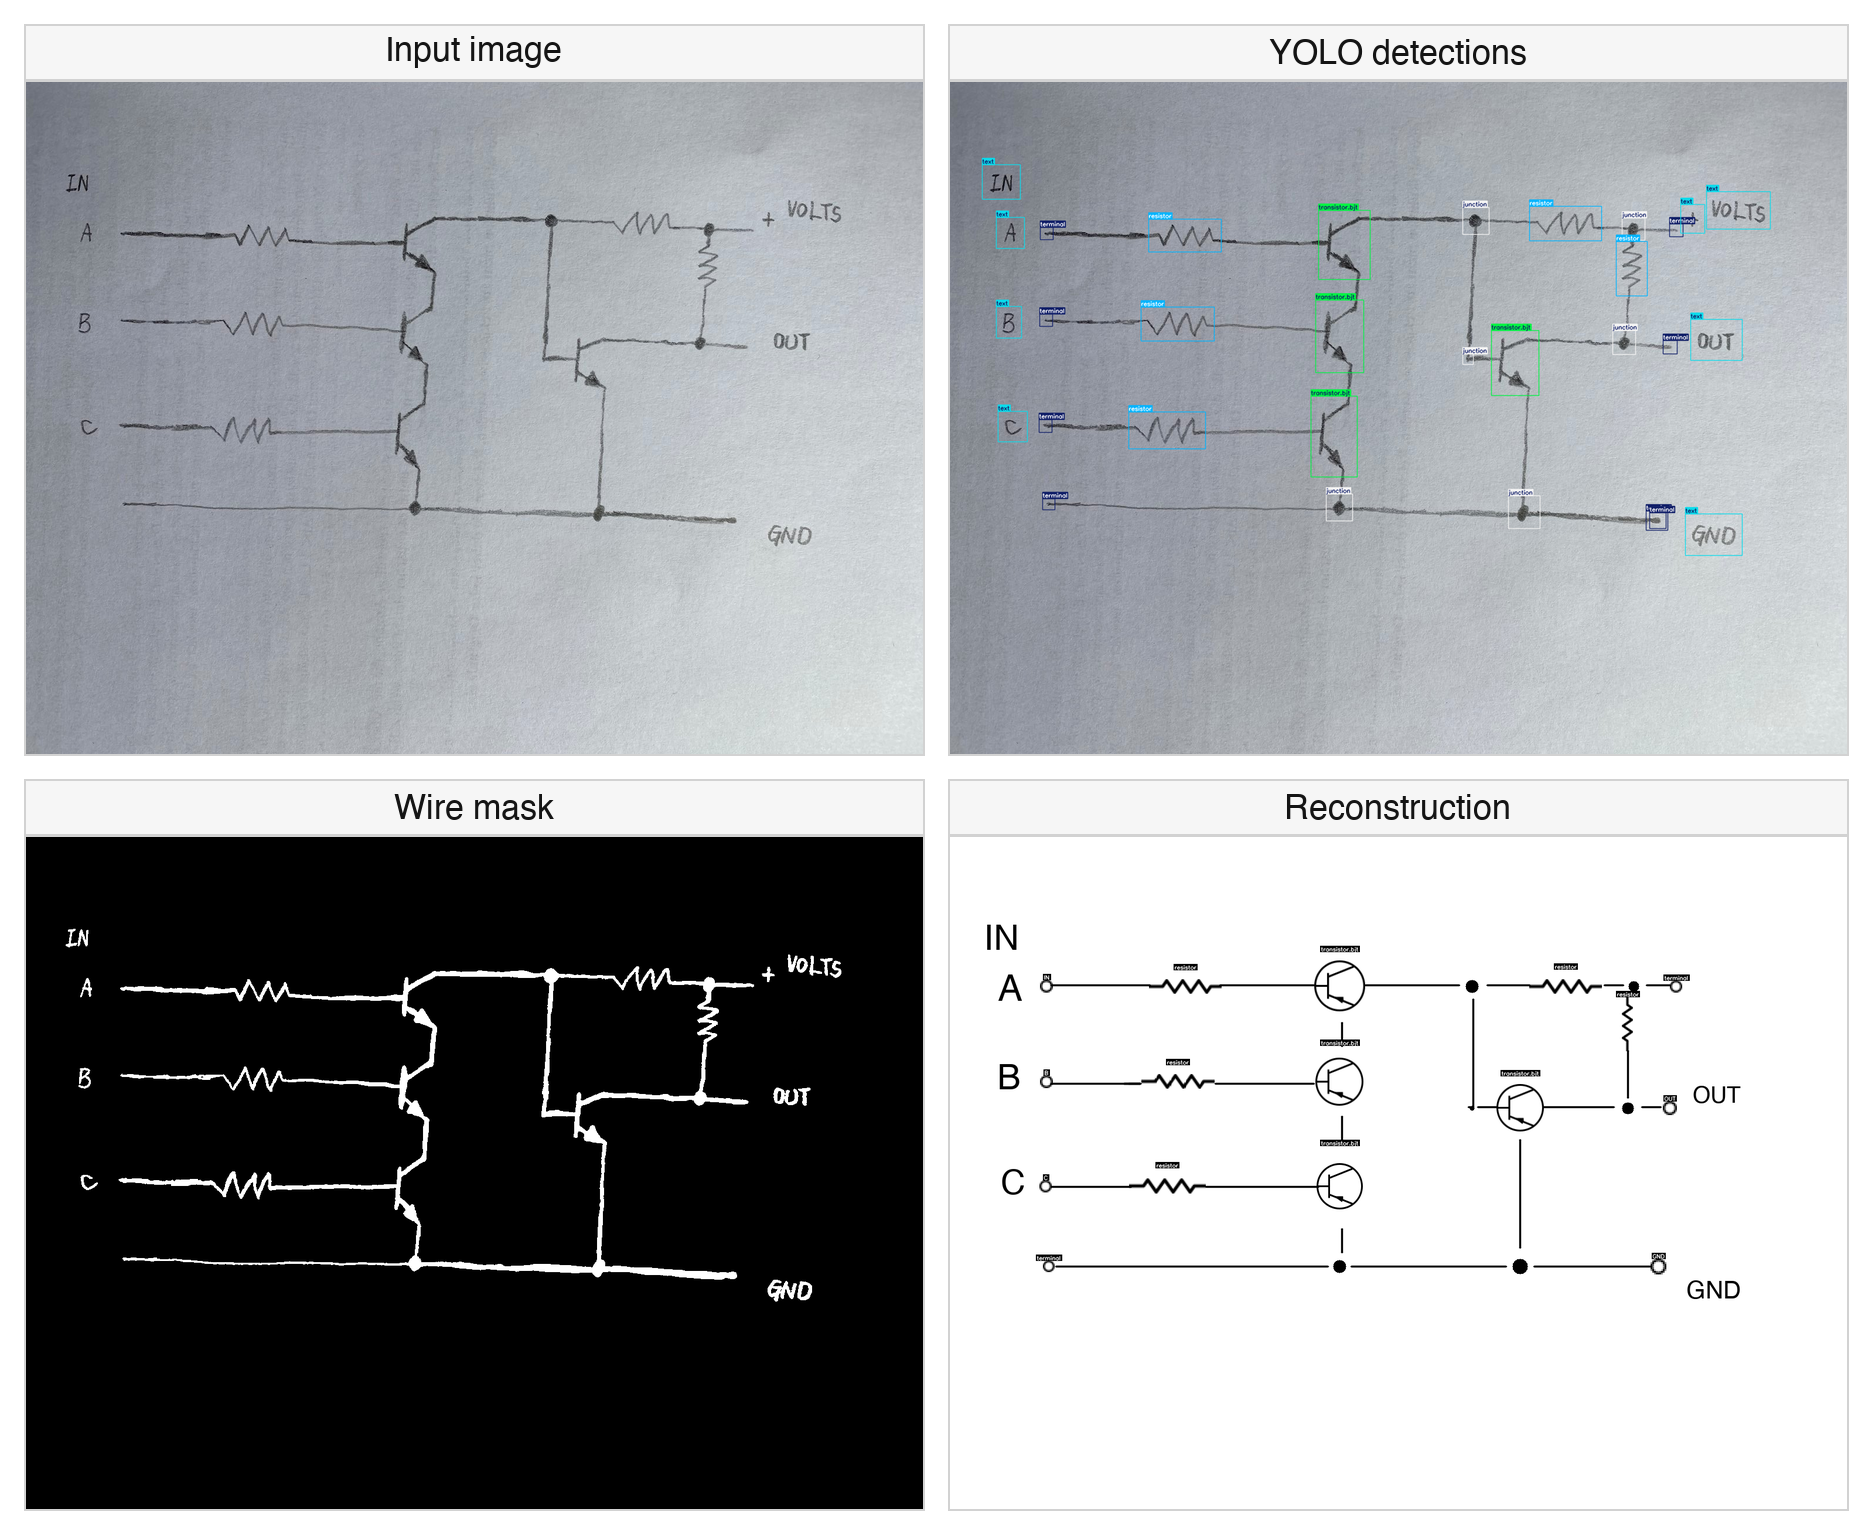
\includegraphics[width=0.95\linewidth]{figures/pipeline.png}
\end{center}
\caption{End-to-end pipeline: YOLO detects components, U-Net segments
wires, TrOCR reads labels, and a rule-based stage assembles an
axis-aligned schematic.}
\label{fig:pipeline}
\end{figure}

The reconstruction stage assembles detections, the wire mask, and OCR
strings into a clean diagram in four steps. First, wire polylines are
extracted from the binary mask by erasing component bounding boxes,
removing small blobs, skeletonizing, and tracing with
\texttt{trace\_skeleton}; polyline endpoints are matched to nearby
component boxes (30\,px margin) to classify each wire as connected,
dangling, or orphan. 

Second, a union-find over wire-induced axis
constraints groups components and snaps each group to its member mean,
correcting cumulative camera-tilt drift that simple pairwise alignment
cannot handle. 

Third, polylines are simplified via Douglas-Peucker
($\varepsilon{=}6$\,px) and projected onto their dominant axis, with
terminal segments snapped to component ports. 

Finally, 17 component classes are rendered from a vector symbol library with orientation
chosen by majority vote of incident wire directions; remaining classes
fall back to labeled bounding-box rectangles.



\section{Discussion and Conclusion}
The pipeline performs well under favorable conditions. On photos taken against plain white paper with good lighting, the reconstructed topology is generally correct and the output is clean. Performance degrades on noisier inputs: heavily annotated schematics in which text labels overlap component symbols, and photos with shadows or background texture, reduce the accuracy of both the detector and the wire segmenter, and these errors compound at the reconstruction stage.

Class imbalance is the dominant data limitation. Seven CGHD classes have fewer than 50 training instances, and augmentation alone was not sufficient to make detection reliable for them. The effect is visible in the final output: missed or misclassified rare components leave gaps in the circuit graph that downstream stages cannot recover.

Reconstruction is the stage most sensitive to upstream errors. A single missed wire segment can disconnect a component from the inferred graph, and the current implementation treats \texttt{crossover} detections as ordinary components rather than as non-connecting wire crossings, which introduces false attachments and distorts the final layout.

Future work should focus on collecting additional real data for rare classes, handling junctions and crossovers explicitly during graph construction, and evaluating alternative wire-tracing and reconstruction methods.
\subsubsection*{References}

\small{
[1] Bayer, J. (2024) \textit{CGHD1152: Collected Graphical Hand-Drawn Dataset of Electrical Schematics.} Kaggle. \url{https://www.kaggle.com/datasets/johannesbayer/cghd1152}

[2] Jocher, G., Chaurasia, A.\ \& Qiu, J. (2023) \textit{Ultralytics YOLO (v8.0).} \url{https://github.com/ultralytics/ultralytics}

[3] Li, M., Lv, T., Chen, J., Cui, L., Lu, Y., Florencio, D., Zhang, C., Li, Z.\ \& Wei, F. (2023) TrOCR: Transformer-based optical character recognition with pre-trained models. In \textit{Proceedings of the AAAI Conference on Artificial Intelligence.}

[4] Ronneberger, O., Fischer, P.\ \& Brox, T. (2015) U-Net: Convolutional networks for biomedical image segmentation. In \textit{MICCAI}, pp.\ 234--241.

[5] Ouyang, T.-Y.\ \& Davis, R. (2009) A visual approach to sketched symbol recognition. In \textit{Proceedings of IJCAI}, pp.\ 1463--1468.

[6] Bresler, M., Van Phan, T., Pr\r{u}\v{s}a, D., Nakagawa, M.\ \& Hlav\'{a}\v{c}, V. (2014) Recognition system for on-line sketched diagrams. In \textit{14th International Conference on Frontiers in Handwriting Recognition (ICFHR)}, pp.\ 563--568.

[7] He, K., Zhang, X., Ren, S.\ \& Sun, J. (2016) Deep residual learning for image recognition. In \textit{CVPR}, pp.\ 770--778.

[8] Bayer, J., van Waveren, L.\ \& Dengel, A. (2024) \textit{Modular Graph Extraction for Handwritten Circuit Diagram Images.} arXiv:2402.11093.
}

\end{document}
